\chapter{Abstract}
\label{chap:abstract}

%rewrite to be more clear?

Birdid.no was developed back in around 2012, back when HTML 5 was still mostly just under development. Things have changed since then. Flash is not longer the only way to display multimedia technologies like sound and video. The web has also moved towards a more mobile friendly environment, leaving flash at the door. This is where our project comes in. The old quiz application on birdid.no is developed in flash, a dying platform. We decided to innovate on this by developing an all new quiz from the ground up in Angular 2. 

The quiz is developed with a combination of Angular 2, bootstrap and Gulp for maximum innovation and results. It intended to bring the quiz in to a new world of standards, frameworks and technologies. It is well known how slow business are innovating and we wanted to change that. The team consist of 4 members, where none was familiar with the framework at the start, but quickly got up to speed. The back-end was handled by Jan Greger, while the entire team worked on the front-end.

The resulting quiz has wide range of features from image quizzes to sound quizzes and beginner quizzes. It even supports most more than 25  languages, formal tests(exams) and personalized competition groups. It also allows users to login for persistent user statistic on all completed quizzes. Each round of quiz consists of one or more questions with a corresponding media and alternatives. The user then can learn to identify birds based on appearance and sound while being assessed by the quiz application. The core of the entire quiz application is the notorious quiz master and quiz component serving most of the content in the quiz. The quiz is a lot more complex than it looks at first glance, something this report want to highlight.




\begin{figure}[h]
  \centering
  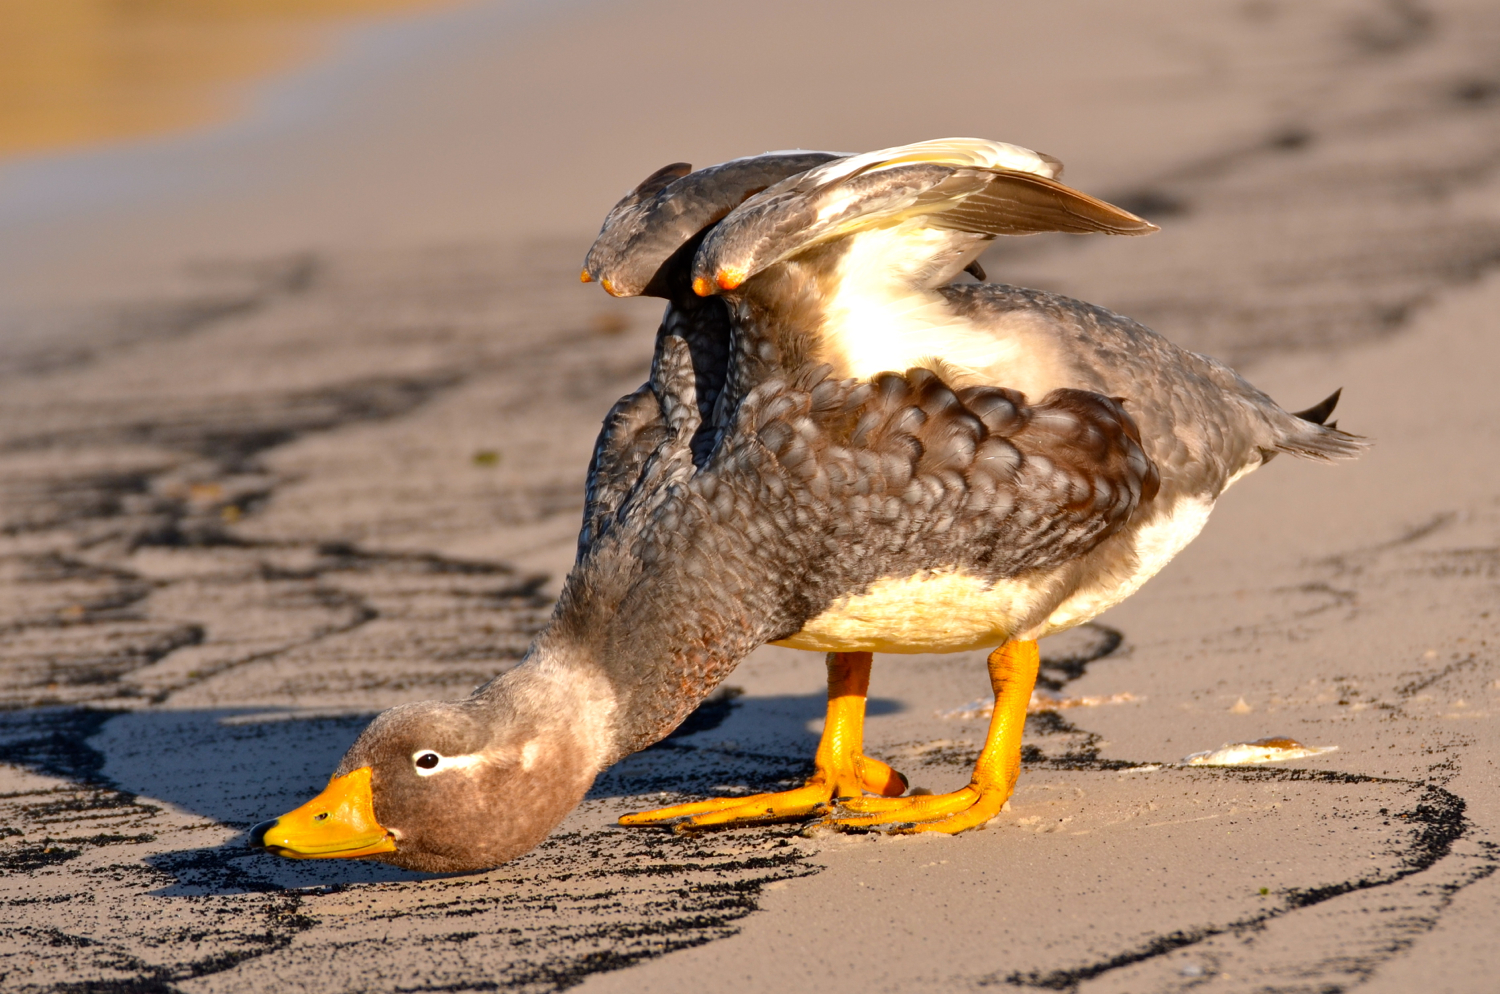
\includegraphics[width=0.5\textwidth]{figures/angbirds.jpg}
  \caption[AngularBird]{An Angular Bird}
  \label{fig:AngularBird}
\end{figure}

